\section{INTRODUCTION}\label{sec:intro}

This work focuses on creating and testing valid trajectories for high degree of freedom (DOF), high-gain, position controlled mechanisms that results in the desired end-effector velocity.  Throwing and hitting are examples of end-effector velocity control.  The goal is to have the end-effector moving at a specific rate in a specific direction.  It is also a task that demands whole-body coordination.  When the arm moves quickly, as in the case of pitching, such upper-body motions, if not coordinated with the lower-body, can cause the humanoid to lose balance.  The overarching goal of this work is to create stable whole-body motions that reliably moves the end-effector at the desired velocity while retaining stability.  Fig.~\ref{fig:huboOneFoot} shows this overarching goal as an example of a stable human like pose when preparing to throw a ball.  The focus of this work is the first required step for throwing with a high gain position controlled robot; throwing an object without self-collision with sparse knowledge of the full reachable area of the robot.  

The resulting system is capable of creating trajectories for overhand and underhand throwing motions.  This work illustrates the trajectory-based approach with underhand throwing, but can also be applied to overhand cases.

\begin{figure}[t!]%[thpb]
  \centering
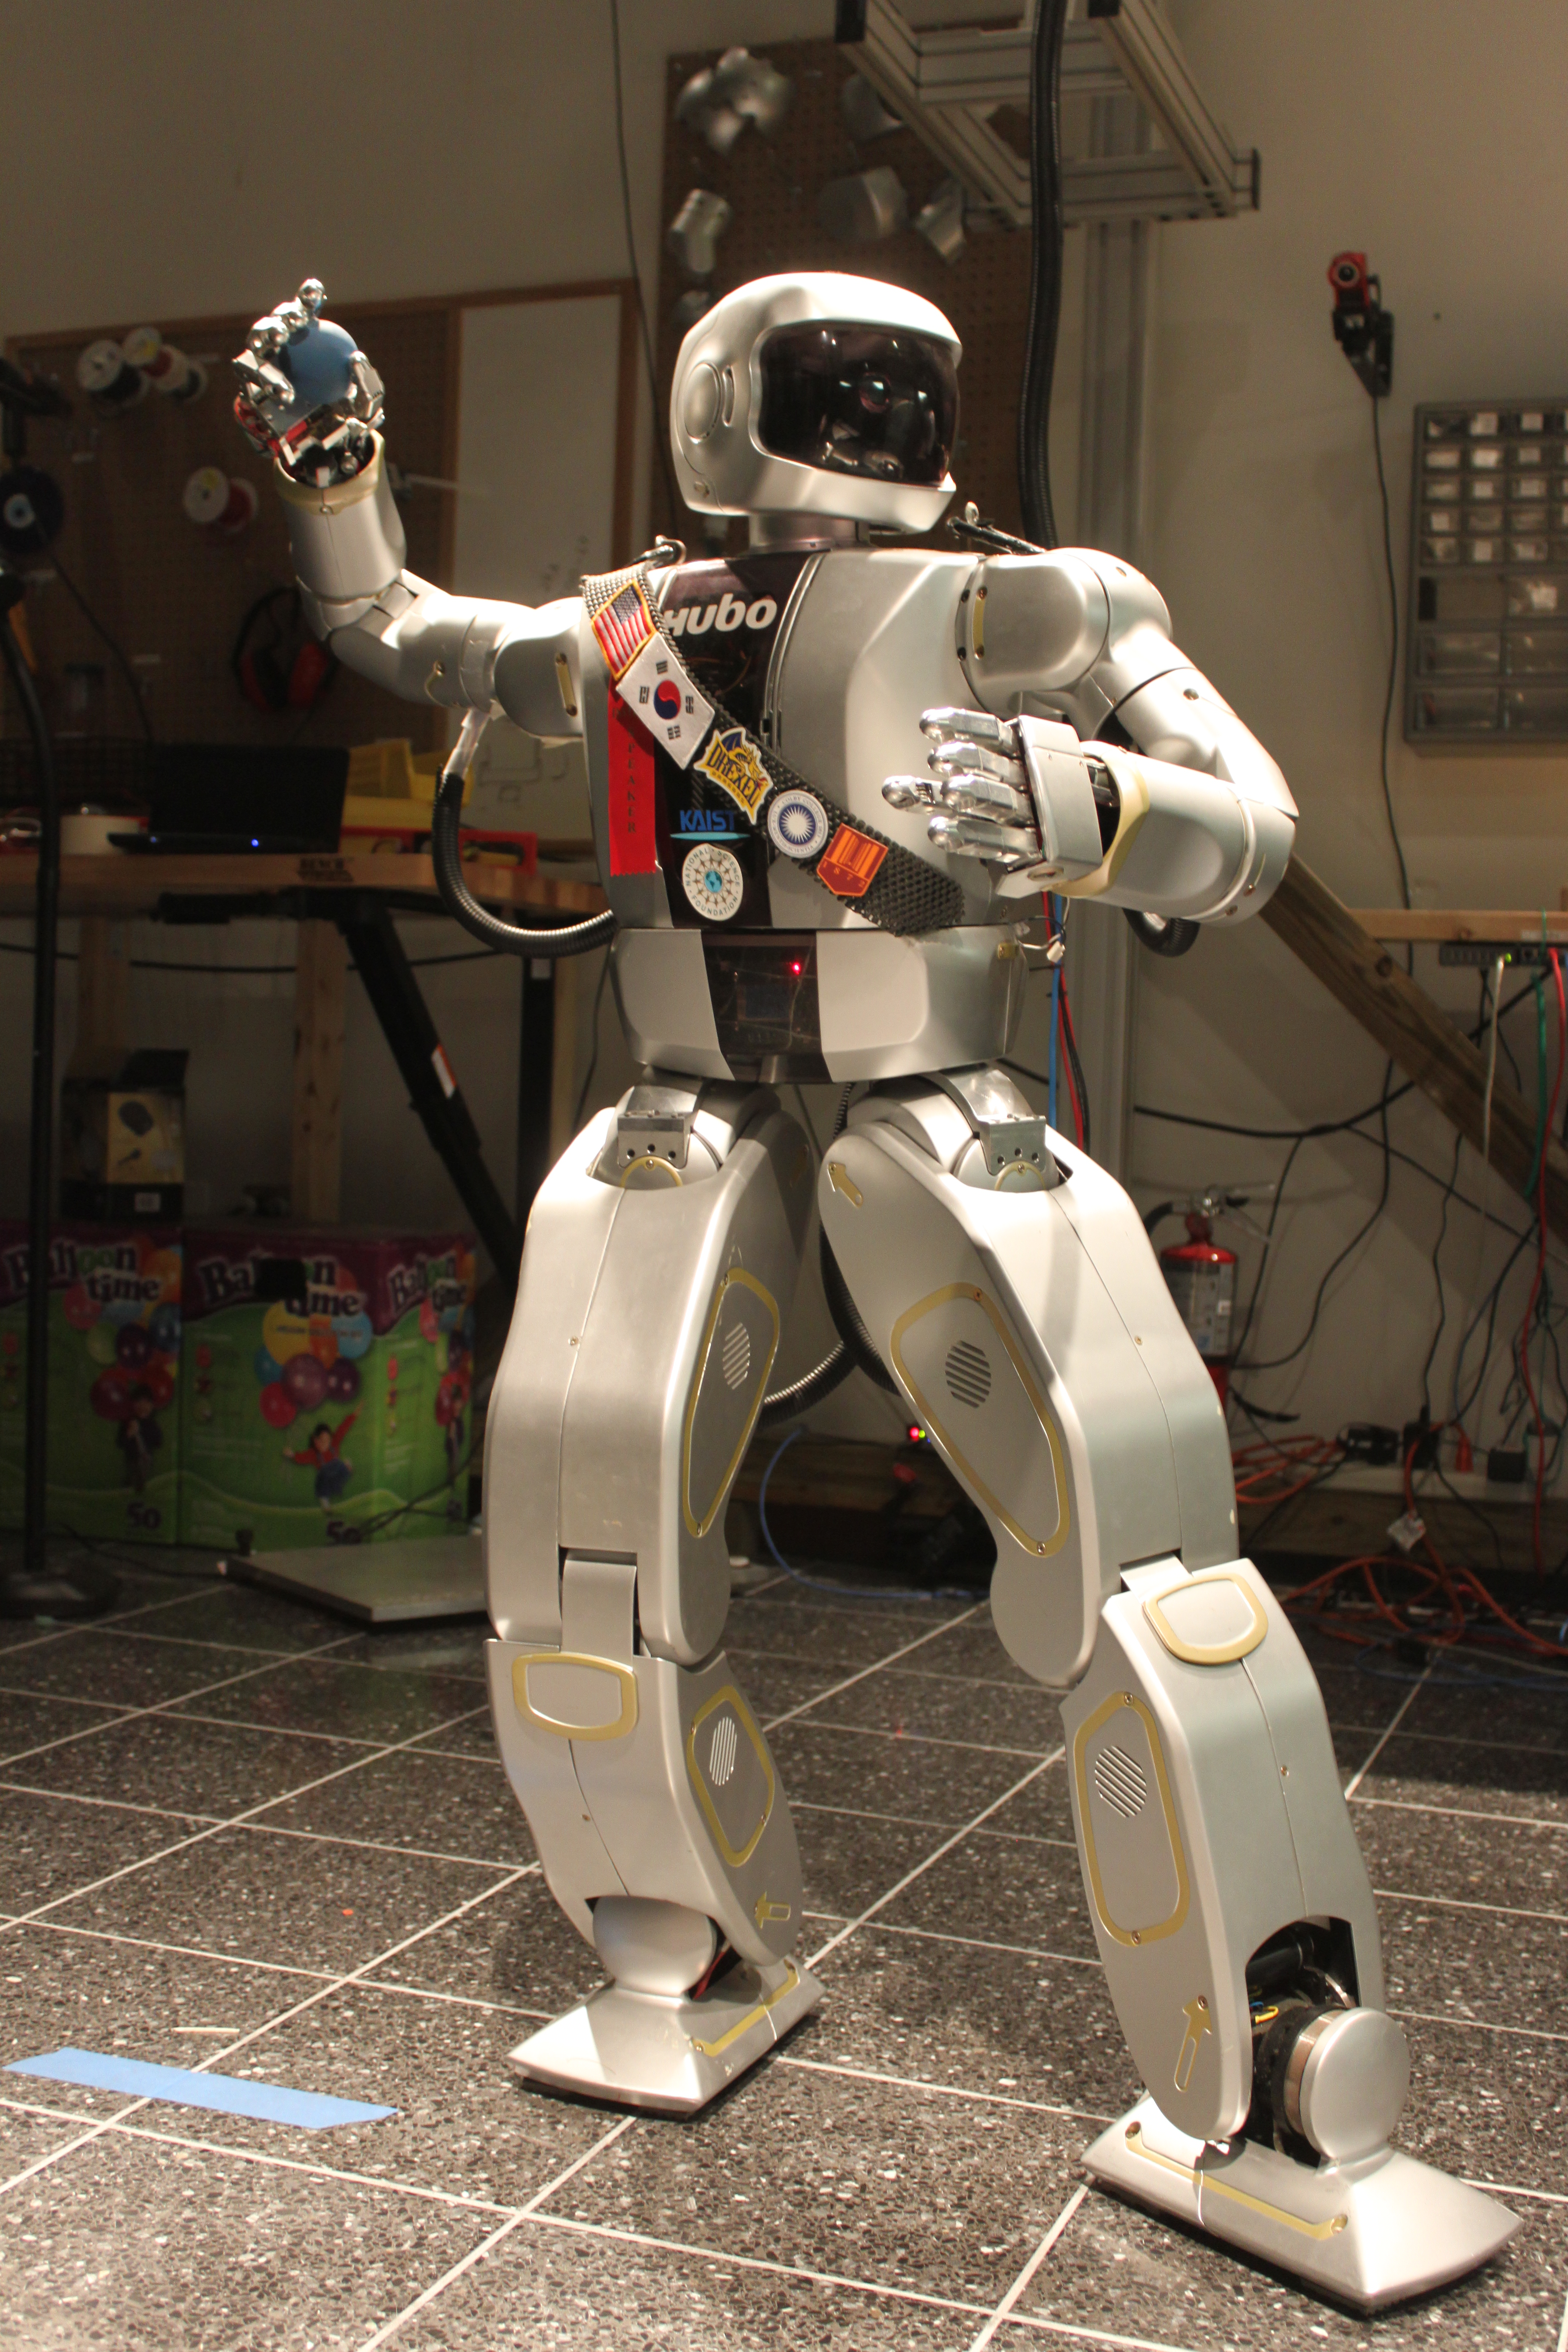
\includegraphics[width=0.55\columnwidth]{./pictures/huboThrow.png}
  \caption{Jaemi Hubo (Hubo KHR-4) demonstrating the initial pose for the overarching goal of creating a full body, human-like, stable, motion for throwing.}
  \label{fig:huboOneFoot}
\end{figure}

The location in space where the desired end-effector velocity occurs is important in instances such as tennis, ping-pong, and other hitting activities where the end-effector does not control the object through out the entire motion.  Throwing is an example of when the end-effector's velocity holds a higher priority over the position.  


Mechanisms with only a single degree of freedom are restricted to throwing in a plane.   2-DOF mechanisms are able to throw in $R^3$ space with the correct kinematic structure.  Such a mechanism can choose its release point or its end-effector velocity but not both.  Mechanisms containing 3 or more DOF with the correct kinematic structure are able to throw in $R^3$ and choose both the release point and the end-effector velocity simultaneously.  

Low degree of freedom throwing machines/robots are common.  Typical throwing robots have between one and three degrees of freedom (DOF)~\cite{509405, Lynch97dynamicnonprehensile, 5152525, 509335, springerlink:10.1007/s10015-006-0401-0}.  All of these mechanisms are limited to throwing in a plane.   Sentoo et al.~\cite{4651142} achieved an end-effector velocity of 6.0 m/s and can throw in $R^3$ space using it's Barret Technology Inc 4-DOF arm with a $360^o$ rotation base yaw actuator.  These low degree of freedom throwing robots are either physically attached/planted to the mechanical ground or have a base that is significantly more massive then the arm.  

Haddadin et al.\cite{6094757} used their 7-DOF arm and a 6-DOF force torque sensor with standard feedback methods to dribble a basket ball.  In addition Zhikun et al.~\cite{6094892} used reinforcement learning to teach their 7-DOF planted robot arm to play ping-pong.  Likewise Schaal et al.~\cite{schaal01/BIRG} taught their high degree of freedom (30-DOF) humanoid robot to hit a tennis ball using on-line special statistical learning methods.  Visual feedback was used in the basketball throwing robot by Hu et al.~\cite{5649335} achieving accuracy an of 99\%.  All of the latter robots were fixed to the ground to guarantee stability.

Kim et al. \cite{5686315,JooH2011438} takes the research to the next level with finding optimal overhand and sidearm throwing motions for a high degree of freedom humanoid computer model.  The model consists of 55-DOF and is not fixed to mechanical ground or a massive base.  Motor torques are then calculated to create both sidearm and overhand throws that continuously satisfies the zero-moment-point stability criteria~\cite{4309277}.  

The highly articulated 40-DOF adult size humanoid robot Jaemi Hubo KHR-4 (Fig.~\ref{fig:huboOneFoot}) is the platform focused on in this work.  Jaemi Hubo is a high-gain, position-controlled biped humanoid robot weighing 37kg and standing 130cm tall.  It is designed and made by Dr. Jun-Ho Oh director of the Hubo Lab at the Korean Advanced Institute of Science and Technology (KAIST).  Jaemi has been located at the Drexel Autonomous Systems Lab (DASL) at Drexel University since Fall of 2008.  DASL has extensive experience with the Jaemi Hubo KHR-4 platform in key areas needed to complete this work.  Balancing was explored when developing a real-time zero moment point (ZMP) preview control system for stable walking~\cite{5686276}.  A full-scale safe testing environment designed for experiments with Jaemi Hubo was created using DASL's Systems Integrated Sensor Test Rig (SISTR)~\cite{5686325}.  Additionally all algorithms are able to be tested on miniature and virtual versions of Jaemi Hubo prior to testing on the full-size humanoid robot through the creation of a surrogate testing platform for humanoid robots~\cite{5379582}.


%  The end-effector position at the desired velocity does not need to be specified.

The goal of this work is to show the creation of collision free trajectories for end-effector velocity control, the first step in our overarching goal of creating a system with the ability to throw objects and retain balance.  Towards this, Section~\ref{sec:selfCollision} will discuss our method of detecting self collisions.  Section~\ref{sec:rarea} describes the creation of the robot's sparse reachable map (SRM), a map in $R^3$ of the reachable points.  Section~\ref{sec:trajGen} shows the creation of a throwing trajectory in $R^3$ and placing it withing the robot's reachable area using the SRM.  Section~\ref{sec:ik} explains the inverse kinematics used to convert the throwing trajectory in $R^3$ to joint space for this high degree of freedom humanoid robot.  Section~\ref{sec:trap} describes the creation of the setup trajectory from the initial pose of the robot to the starting pose of the throwing trajectory using a variant of trapezoidal motion control to keep within the actuators' physical limitations.  Section~\ref{sec:exp} features experiments to demonstrate the successful execution of this paper's goal of throwing.  Section~\ref{sec:conc} concludes the paper and comments on future work.

%The goal of this work is to show the creation of collision free trajectories for end-effector velocity control, the first step in our overarching goal of creating a system with the ability to throw objects and retain balance.  Towards this, Section~\ref{sec:selfCollision} will discuss our method of detecting self collisions.  Section~\ref{sec:rarea} describes the creation of the robot's sparse reachable map (SRM), a map in $R^3$ of the reachable points. through setting random values to the robot in joint space that takes into account joint limitations and self collisions.  Section~\ref{sec:trajGen} shows the creation of a throwing trajectory in $R^3$ and placing it withing the robot's reachable area using the SRM.  Section~\ref{sec:ik} explains the inverse kinematics used to convert the throwing trajectory in $R^3$ to joint space for this high degree of freedom humanoid robot.  Section~\ref{sec:trap} describes the creation of the approach from the initial pose to the starting pose of the throwing trajectory using a variant of trapezoidal motion control to keep within the actuators' physical limitations.  Section~\ref{sec:exp} features experiments to demonstrate the successful execution of this paper's goal.  Section~\ref{sec:conc} concludes the paper and comments on future work.